
\chapter{Experiments}
\label{experiments}

Both long- and short-term prediction and forecasting experiments were considered, as well as both neighborhood level spatial granularity and a larger city level scheme. A summary of each is provided in the table below:

\begin{table}[h!]
\centering
\caption{Models Considered}
\label{model_summary}
\begin{tabular}{@{}llllll@{}}
\toprule
Outlook     & Spatial Feature & Frequency & Fitting Period & Look-Ahead Period & Stationary \\ \midrule
Long-Term   & None            & Weekly    & 3 years        & 52 Weeks          & No         \\
Medium-Term & Neighborhoods   & Weekly    & 1 year         & 26 Weeks          & Yes        \\
Short-Term  & Grid Squares    & Weekly    & 6  weeks       & 12 Weeks          & Yes        \\ \bottomrule
\end{tabular}
\end{table}

\section{Data}

The experiments used observational administrative data gathered as part of New York City's Open Data civic reporting system \cite{mvc}. There are many recorded urban events outside of the aforemented policing context where predictive and forecasting knowledge could be helpful to resarch, policy, or operations. Quality-of-life programs such as noise abatement, pest control, and traffic reduction are all natural candidates where data is already collected from the public; in New York City it is done through the 311 civil reporting system. Each also involves allocating scarce public resources e.g., public safety officers, exterminators, and health inspectors over space and time. \par

Although the aforementioned urban events are ex-ante all topic of interests with some potential for spatiotemporal forecastability and would benefit from more accurate modelling, this project instead focused on another heavily spatially dependent public safety issue: vehicle collisions. There have been over 200 fatalities annually resulting from vehicle collisions in New York City over the past five years while Mayor Bill de Blasio's Vision Zero plan has publicly stated a goal of lowering the number of fatalities to zero \cite{nyc_vz}. \par

While approximately 200 fatalities a year is not a 'rare' event, the likelihood of observing a fatality at any given time and place in New York City is exceedingly rare. What's more, public safety interventions in the form of increased enforcement or street redesign can be deployed reactively to the scene of a fatality with little or no information about the relative risk of that location. \par

By contrast, non-fatal injuries resulting from traffic collisions are much more common, with X in 2017 alone where Y of them were marked as serious \todo{fill in injury stats}. By thinking of injuries as a potential fatality observing and attempting to forecast these injures reliably could provide a much better estimate of where the city is particularly risky for traffic collisions. These estimates could in turn be used to evaluate the efficacy of any public safety intervention after the fact instead of relying on observing only the future fatality count which may be subject to mean reversion in a situation where the mean fatalities at any given place and time are very close to zero. Since vehicle collisions are reported directly by responding public safety personnel they are not subject to the reporting bias it would be plausible to find in complaint/report data like 311, which would have added an additional source of potential bias.\par

\subsection{Data Processing}

Organizing spatiotemporal count data into a suitable form for modelling presents a challenge in itself. While every count observation occured at a specific point and time, aggregating to a form appropriate both for modelling and capable of providing useful granular forecasts is a balancing act. Traffic collisions in particular are difficult to aggregate into consistent spatial locations that also have a coherent interpretation of the distance between each location necessary for fitting a spatiotemporal model. \par

There are many administrative spatial aggregation bounds which are of potential use, such as Neighborhoods, Zip Codes, Census Blocks, or even unique street intersection IDs. While all may be perfectly viable depending on the situation, gridding provides a more generalizable spatial aggregation method which is already used in many spatial statistics applications, see for example the case studies in \cite{blangiardo_2015}. Gridding simply overlays a square grid of chosen size on the area of interest and sums all the count data within each grid cell into a single data point, a flexible method that can be easily - if imperfectly - applied to many spatial contexts. Being able to flexibly choose the size of grid squares adds an additional layer of modelling flexibility. \par

Finally gridding offers clear benefits in the specific case of Gaussian process models. Since the spatial kernel $k_s$ calculates the distance between any point $s_i$ and all other points in $s$ the computational cost of adding an additional point in $s$ is high. By specifying the distance calculation only between the centroid of each grid square this method at least offers an explicit choice between higher spatial resolution and computational complexity.


\begin{figure}[h!]
  \centering
  \caption{A grid of 1250ft grid squares overlaid on the Park Slope street grid.}
  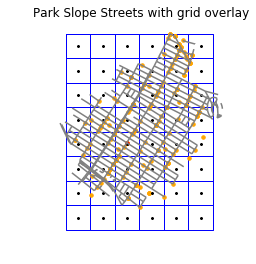
\includegraphics[\textwidth]{PS_street_grid}
\end{figure}

\section{Kernel Choice}

The kernel types specified for each $k$ differed slightly from Flaxman 2014 after experimenting with various configurations. Table \ref{kernel_summary} describes the kernel combinations used for each model. Other combinations were considered, including using variations of the Matern class and varying the interaction term, but none exhibited better performance.


\begin{table}[]
\centering
\caption{Kernel Specifications}
\label{kernel_summary}
\begin{tabular}{@{}llllll@{}}
\toprule
            & Temporal & Spatial  & Periodic & Product            & Linear \\ \midrule
Long-Term   & RBF      & No       & Yes      & No                 & Yes    \\
Medium-Term & RBF      & Matern32 & Yes      & Spatial x Temporal & No     \\
Short-Term  & RBF      & RBF      & Yes      & Spatial x Temporal & No     \\ \bottomrule
\end{tabular}
\end{table}


\section{GPflow}

GPflow is a Python package developed for fitting Gaussian Process models that takes advantage of the gradient methods of Google's TensorFlow to generate Maximum-A-Posteriori (MAP) estimates of the posterior distribution \cite{GPflow2017} \cite{tensorflow2015-whitepaper}. All models are converted into tensors and passed to Tensorflow's optimization algorithms that can run on Graphics Processing Units (GPUs) for fast and efficient computation. This cuts the time needed for each iteration significantly compared to running on a CPU and also doesn't restrict the user to using conjugate distributions when specifying priors and likelihoods - a prerequisite for the LGCP model. GPflow is also capable of full Bayesian inference using Hamiltonian Monte Carlo (HMC), but is currently only available experimentally.

\subsection{Custom Modifications}

While GPflow offers most of the settings required 'out-of-the-box', a few additional features had to be added independently. The base package does not offer the option for a Student-T prior, which was relatively easy to add by writing a new custom Student-T class to GPflow. The package also by default does not easily allow for decomposition of the different kernels' contribution to the parameter estimates. Finally, the GPflow implementation of Matern kernels often exhibit unstable behavior, even after re-centering data. A small jitter was added to the Matern32 kernel in in order to reduce the chance of the Cholesky decomposition failing. All modifications can be found in the appendix \ref{AppendixC}.
